\documentclass{article}
\usepackage{graphicx}
\usepackage{subcaption}
\usepackage{siunitx}

% \usepackage{fancyhdr}
\usepackage[a4paper,width=180mm,top=15mm,bottom=15mm]{geometry}

% \pagestyle{fancy}
% \fancyhf{}
% \rhead{
\includegraphics[width=2cm]{uliege_logo.png}} % Replace 'example-image' with the filename of your image

% \title
% {
%     
\includegraphics[width=5cm]{pics/uliege_logo.png}\\[1cm]

%     \textbf{MATH0001: Communication Graphique}
%     \large Université de Liège - Faculté des sciences appliquées
%     }

% \author{Étudiant: Alexandre Detienne\\
% Matricule ULiege: s2301654}

% \date{20 Décembre 2023}
\begin{document}

\begin{titlepage}
    \begin{flushleft}
        
\includegraphics[width=6cm]{pics/uliege_logo.png}
    \end{flushleft}
    \begin{center}
        \vspace{2cm}

        \LARGE{\textbf{MATH0001: Communication Graphique}}

        \vspace{0.5cm}

        \large{Université de Liège - Faculté des sciences appliquées}

        \vspace{0.5cm}

        \begin{tabular}{l l}
            Étudiant: & Alexandre Detienne\\
            \\
            Matricule: & s2301654\\
        \end{tabular}

        \vspace{2cm}

        \LARGE{\textbf{Projet-examen:} Train d'atterissage de Corsair}

        \vspace{1cm}

        Rapport
    
        \vspace{1.5cm}

        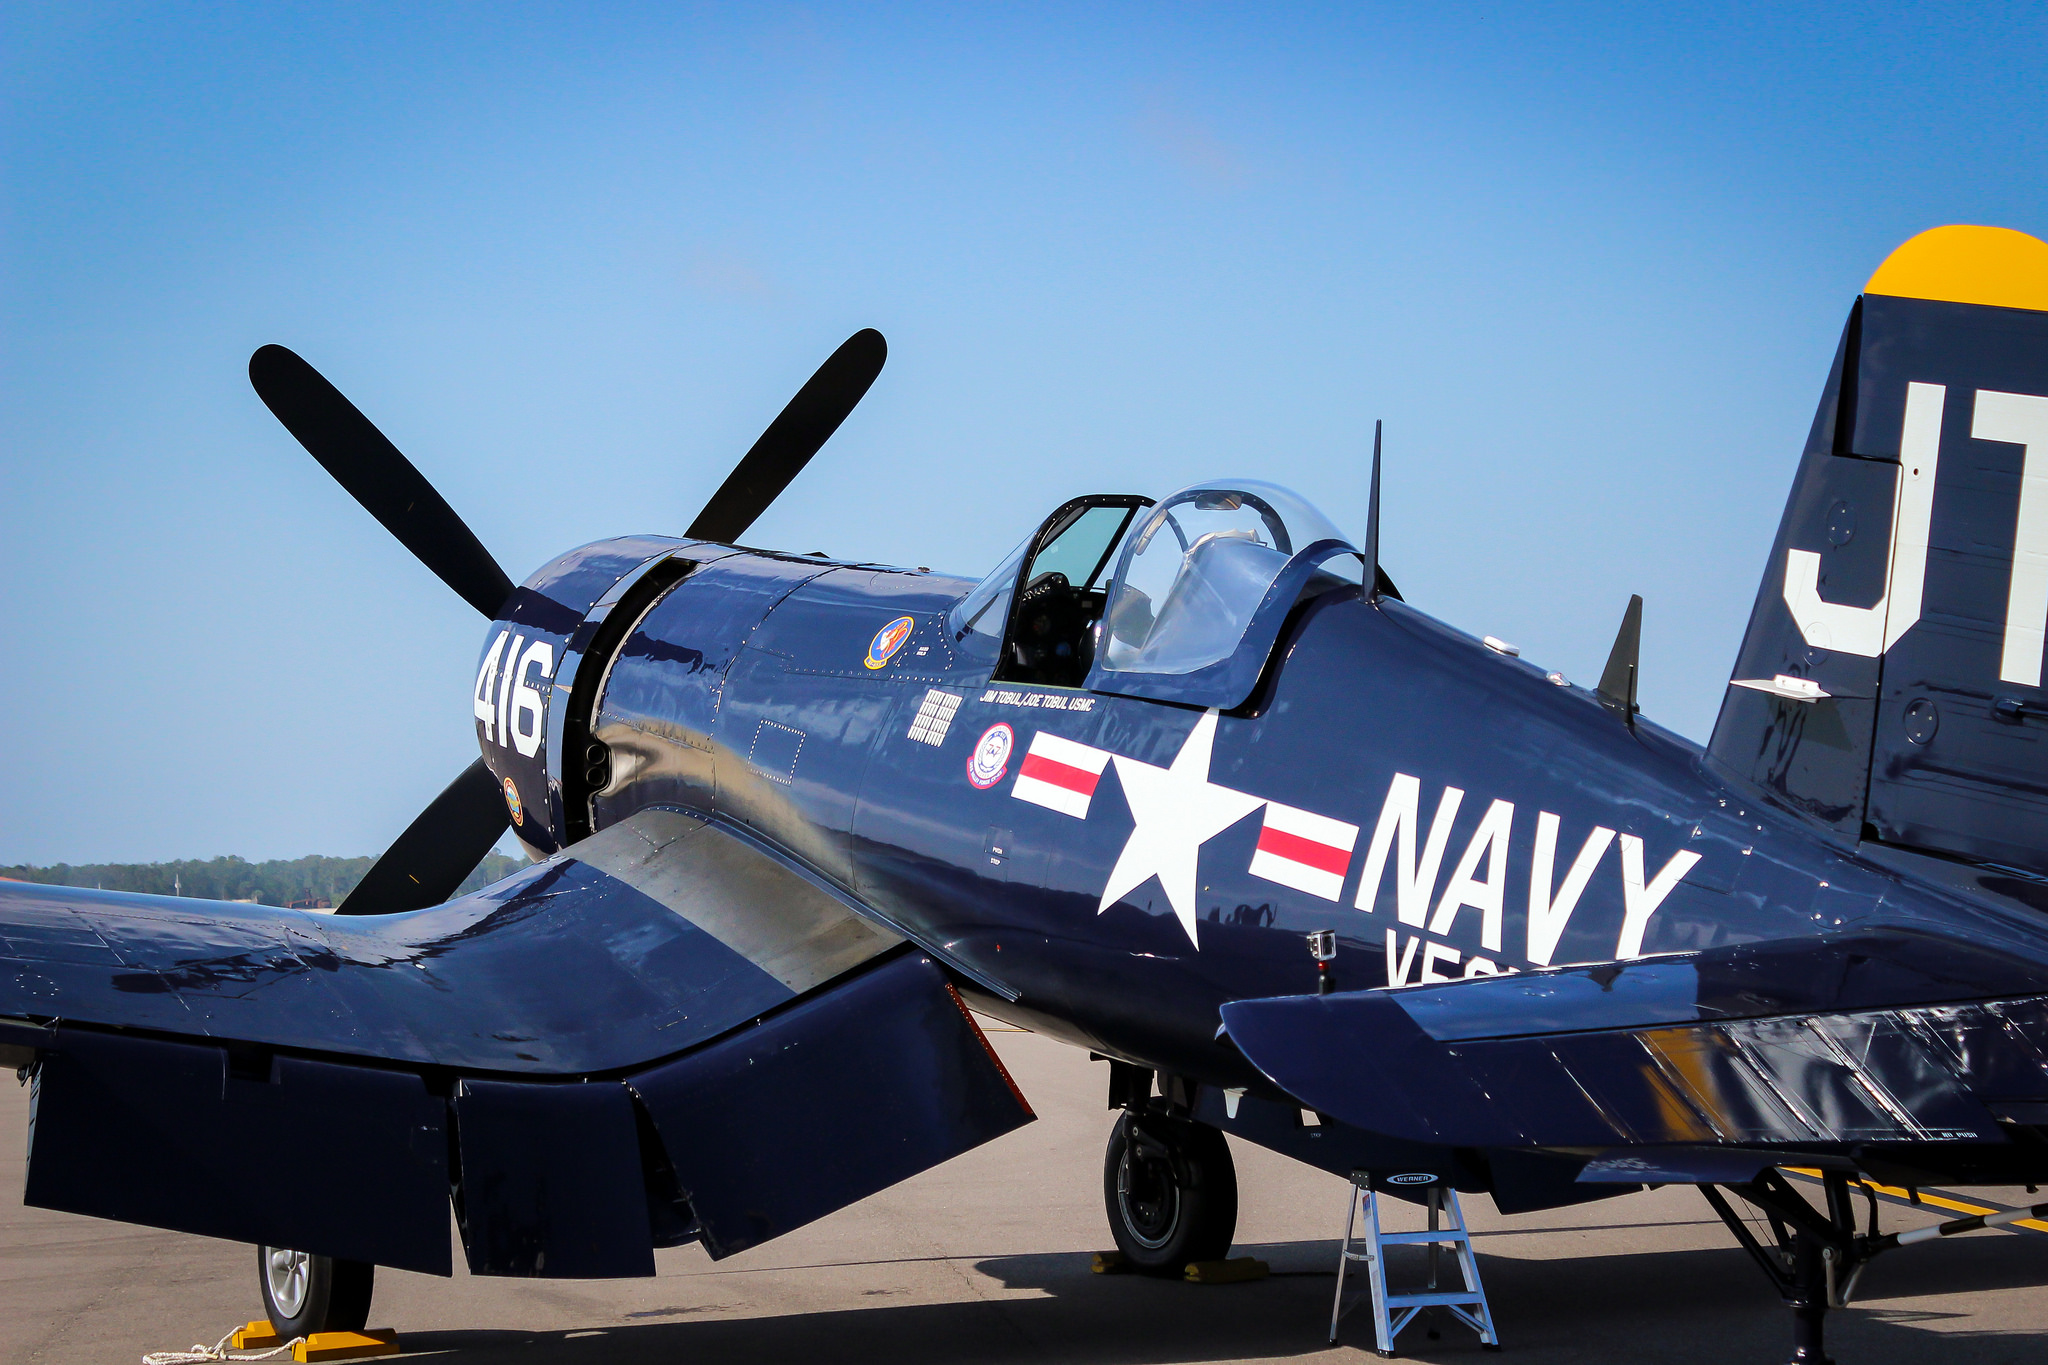
\includegraphics[width = 0.8\linewidth]{pics/corsair_image_frontpage.jpg}

        \vspace{1cm}
    \end{center}

    \begin{flushleft}
        Année Académique 2023-2024

        NX22 - Alexandre Detienne - Décembre 2023
    \end{flushleft}
\end{titlepage}

\newpage
% \tableofcontents

\newpage
\section{Données du modèle paramétrique}
Les paramètres qui ont été affectés à mon matricule étudiant (S2301654) sont
\begin{center}
    \begin{tabular}{|c|c|c|}
        \hline
        M1 & M2 & M3\\
        \hline
        4 & 5 & 6\\
        \hline
    \end{tabular}
\end{center}

\section{Analyse des résultats}
\subsection{Rotation de la roue}

En faisant se déployer le train sur une durée de 20 secondes, on provoque la rotation de l'amortisseur selon son axe longitudinal, ce qui entraine une rotation de la roue autout de cet axe. Sur la figure \ref{fig:wheel_rotation}, on peut voir la position de la roue complètement abaissée en \(t = 0\) (fig~\ref{fig:wheel_down_t0}), et complètement relevée en \(t=20\) (fig~\ref{fig:wheel_up_t20}).

\begin{figure}[h]
    \centering
    \begin{subfigure}[h]{0.48\textwidth}
        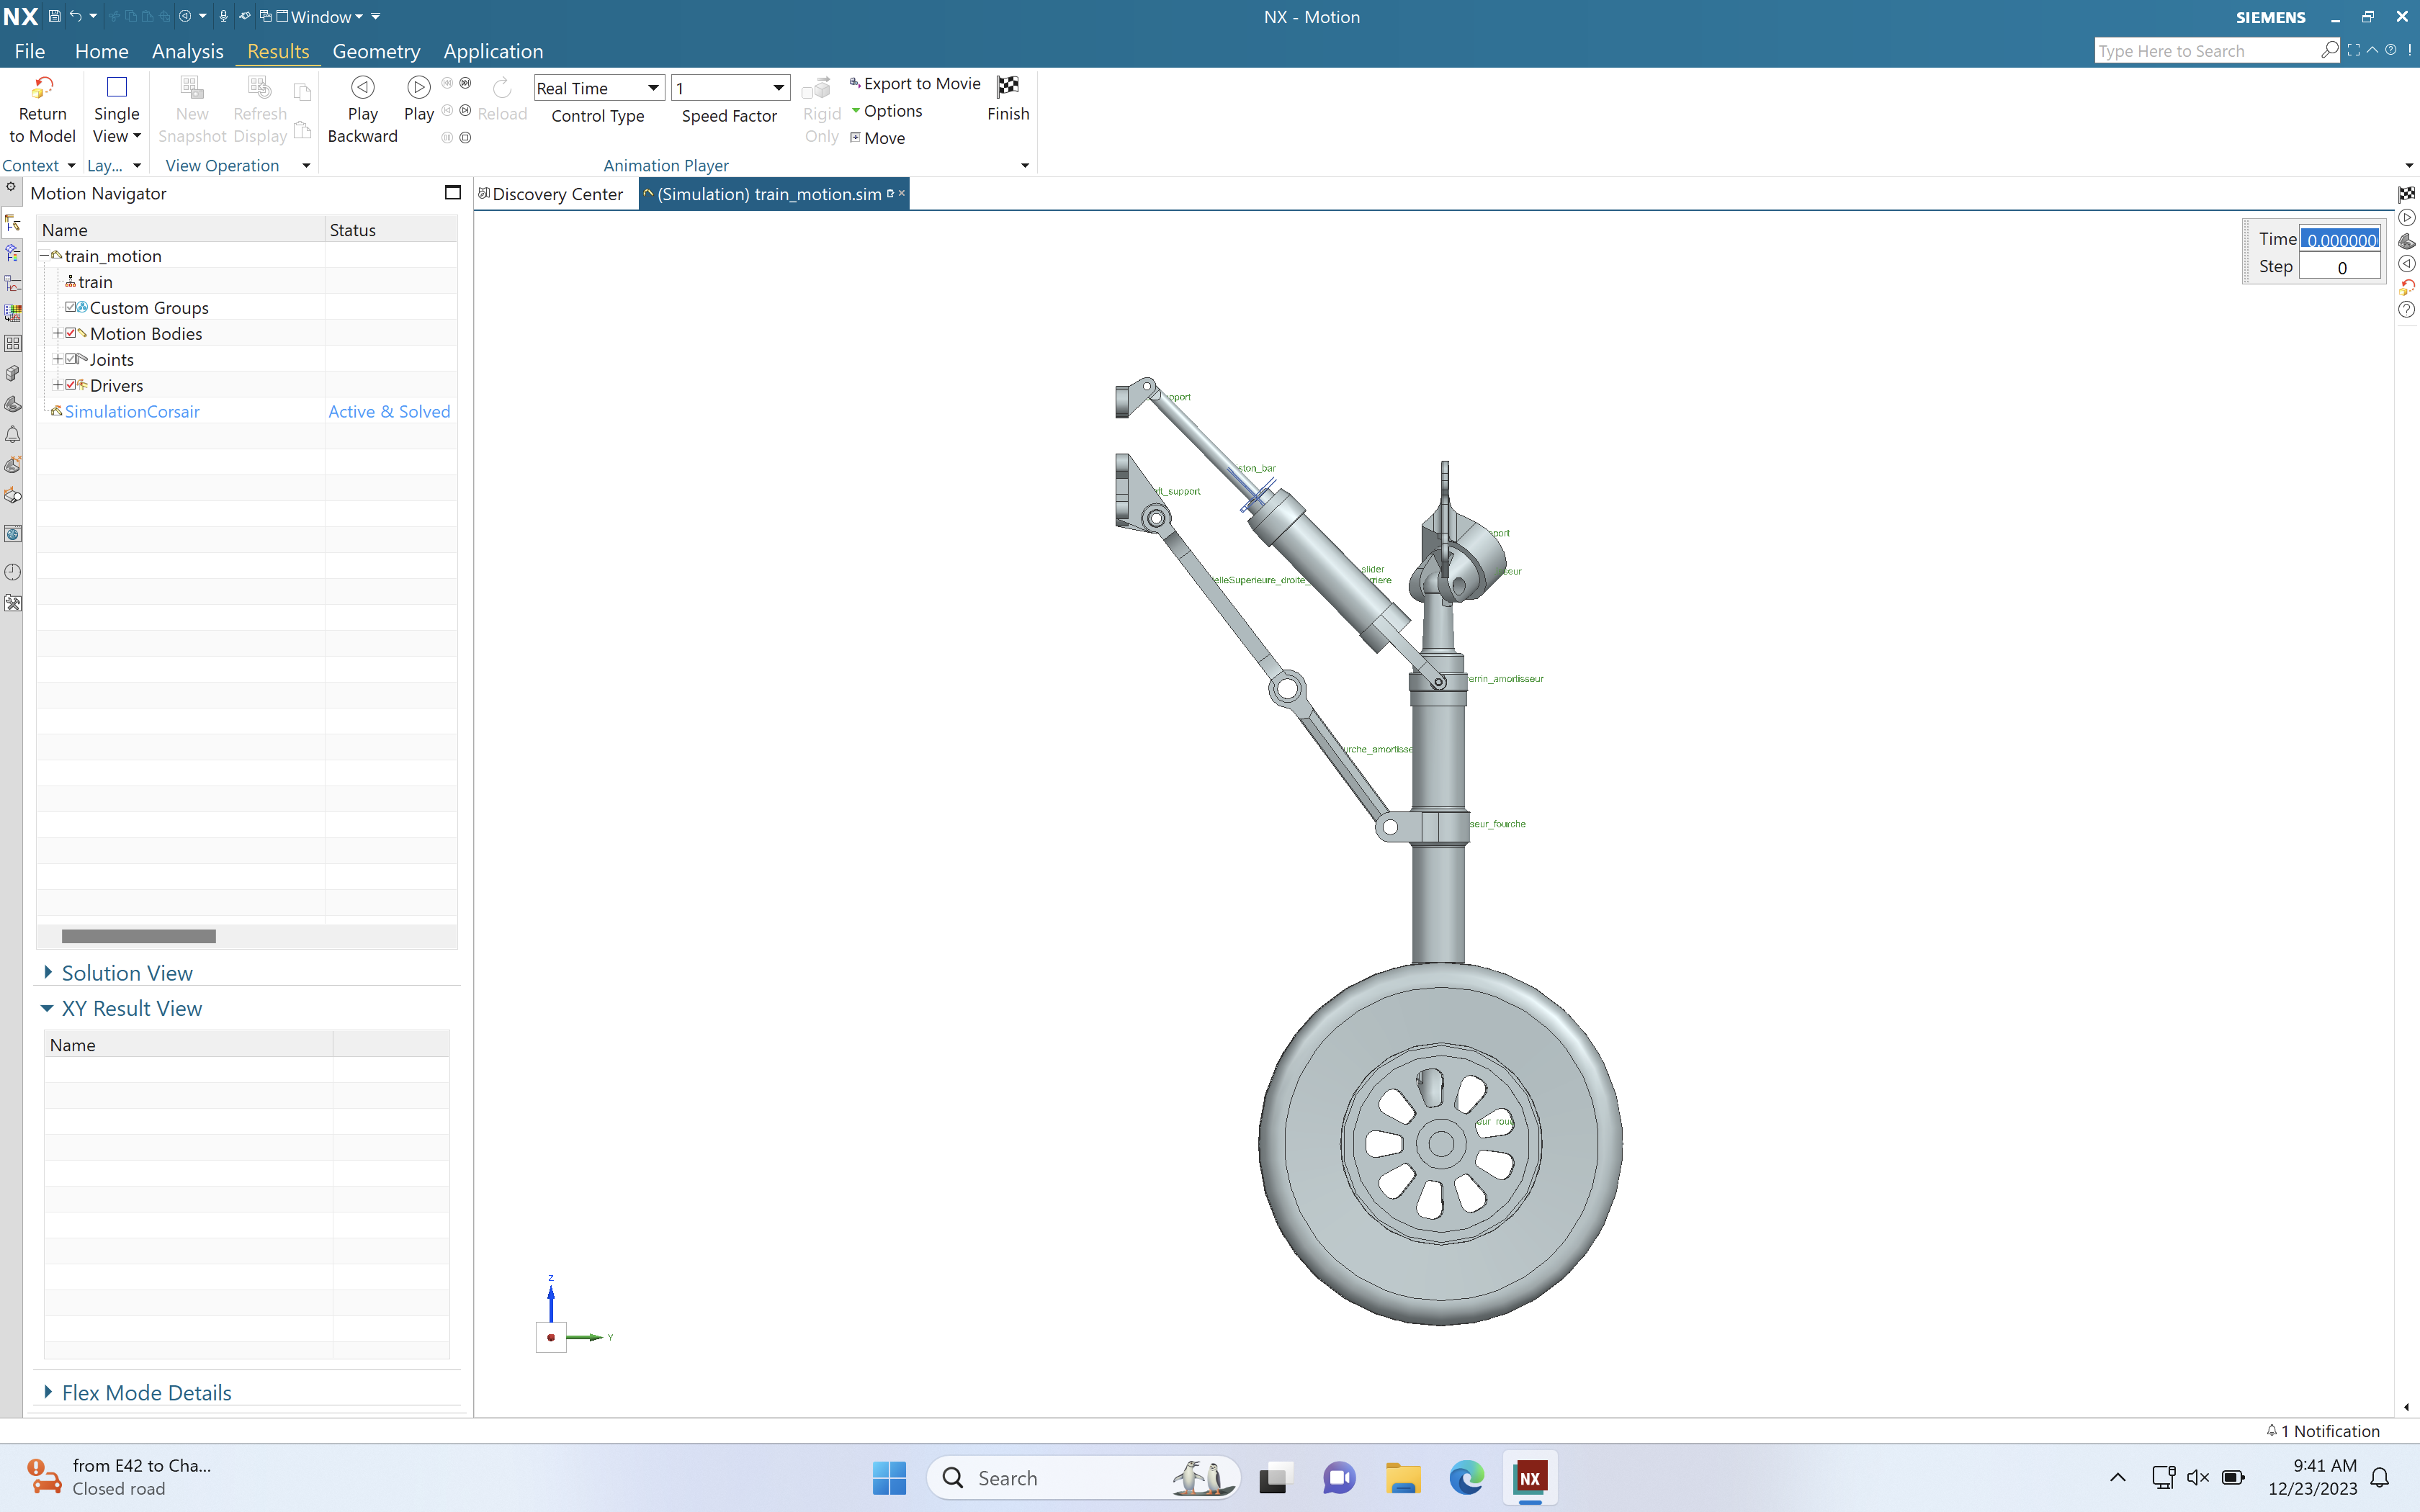
\includegraphics[width=\textwidth]{pics/wheel_down_t0.png}
        \caption{Position de la roue au temps initial (t=0)}
        \label{fig:wheel_down_t0}
    \end{subfigure}
    \hfill
    \begin{subfigure}[h]{0.48\textwidth}
        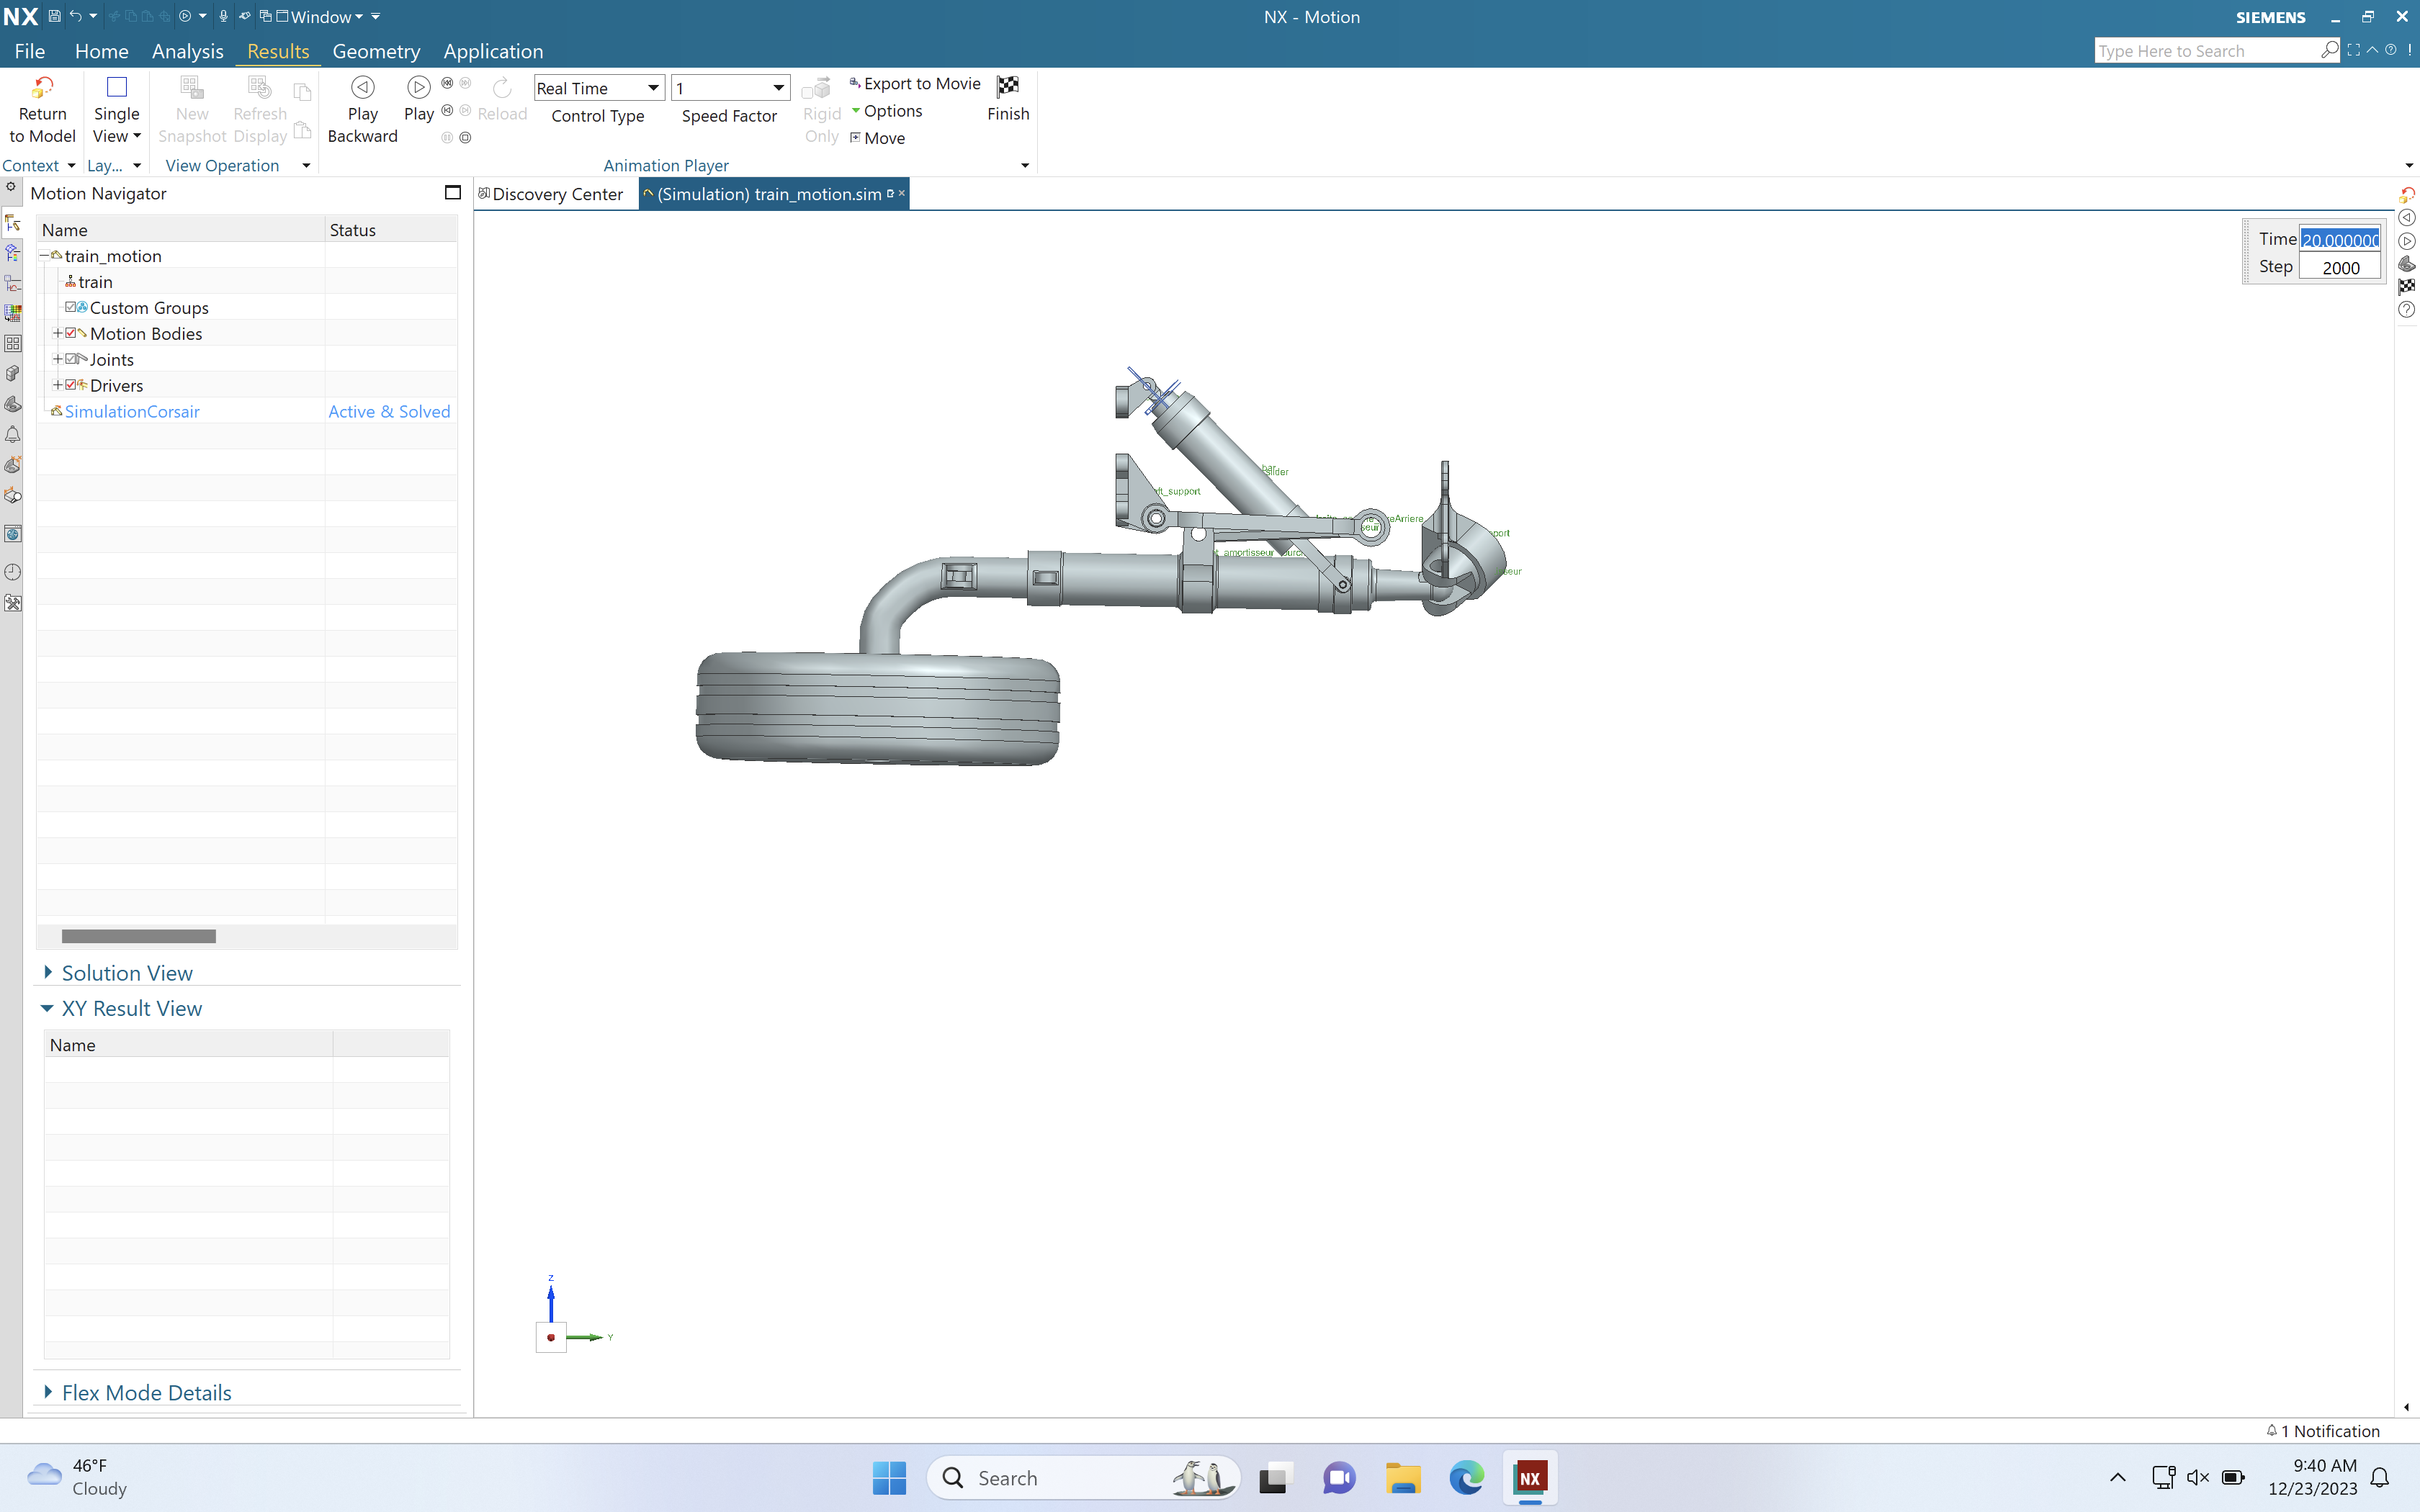
\includegraphics[width=\textwidth]{pics/wheel_up_t20.png}
        \caption{Position de la roue au temps final (t=20)}
        \label{fig:wheel_up_t20}
    \end{subfigure}
    \caption{Visualisation de la rotation de la roue autour de l'axe de l'amortisseur}
    \label{fig:wheel_rotation}
\end{figure}

Comme on peut le voir sur la figure~\ref{fig:wheel_rotation_angle}, la roue aura pivoté de 88.3 degrés à la fin du mouvement de rétractation du train d'atterissage, ce qui est dans les tolérances acceptées pour l'exercice.
\begin{figure}[h]
    \centering 
    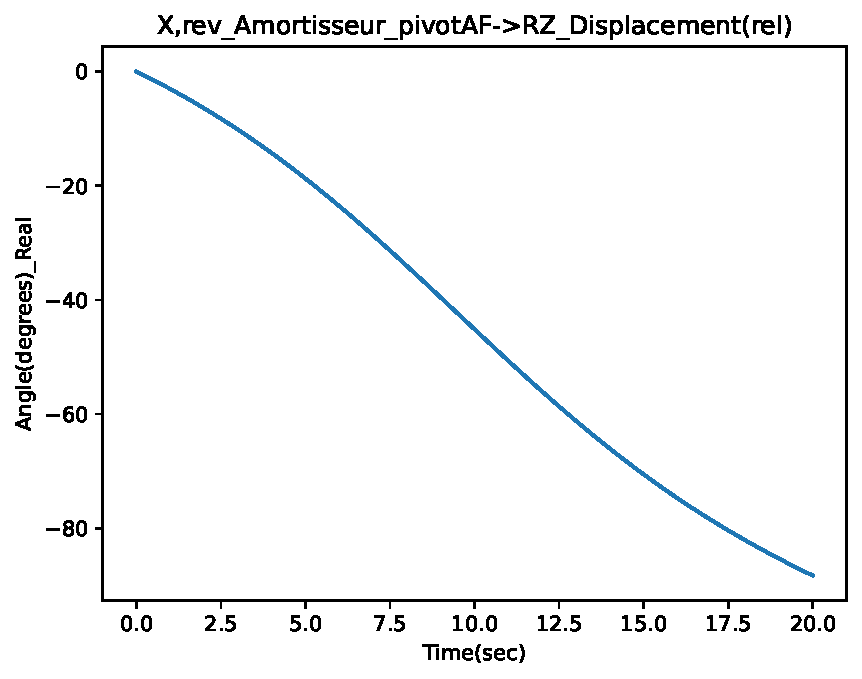
\includegraphics[height=8cm]{data/displacement_angle_amortisseur.pdf}
    \caption{Angle de rotation de la roue en fonction du temps}
    \label{fig:wheel_rotation_angle}
\end{figure}

\pagebreak
\subsection{Vitesse et accélération angulaire de l'axe principal}

La figure~\ref{fig:rot_vel_accel_axe_principal} montre la vitesse angulaire du joint par rapport à l'axe z (figure~\ref{fig:velocity_main_axis}) et l'accélération angulaire correspondante (figure~\ref{fig:accel_main_axis}).
\begin{figure}[h]
    \centering
    \begin{subfigure}[h]{.48\textwidth}        
        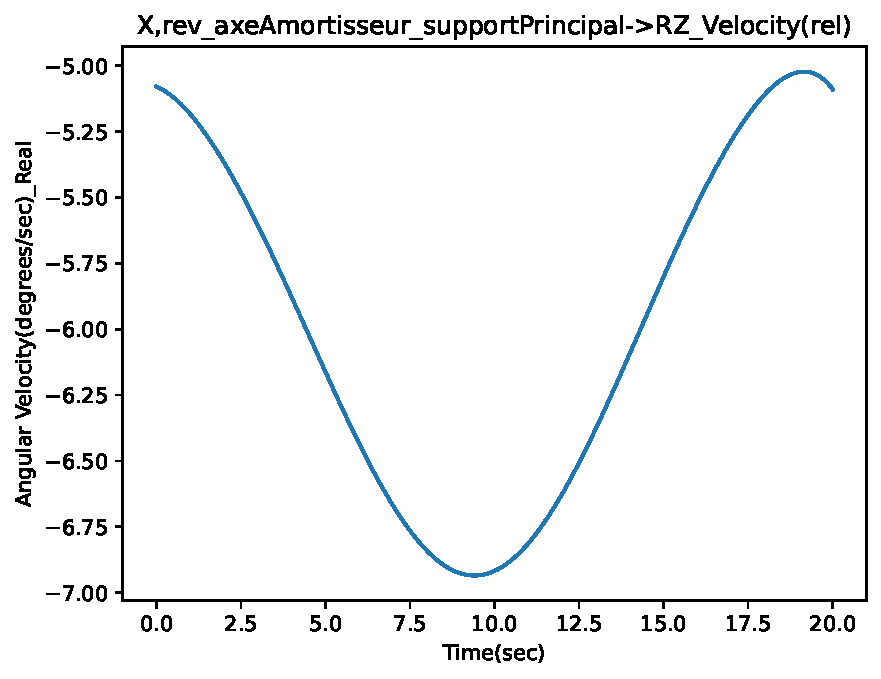
\includegraphics[width=\textwidth]{data/velocity_axeAmortisseur.pdf}
        \caption{Vitesse angulaire}
        \label{fig:velocity_main_axis}
    \end{subfigure}
    \hfill
    \begin{subfigure}[h]{.48\textwidth}        
        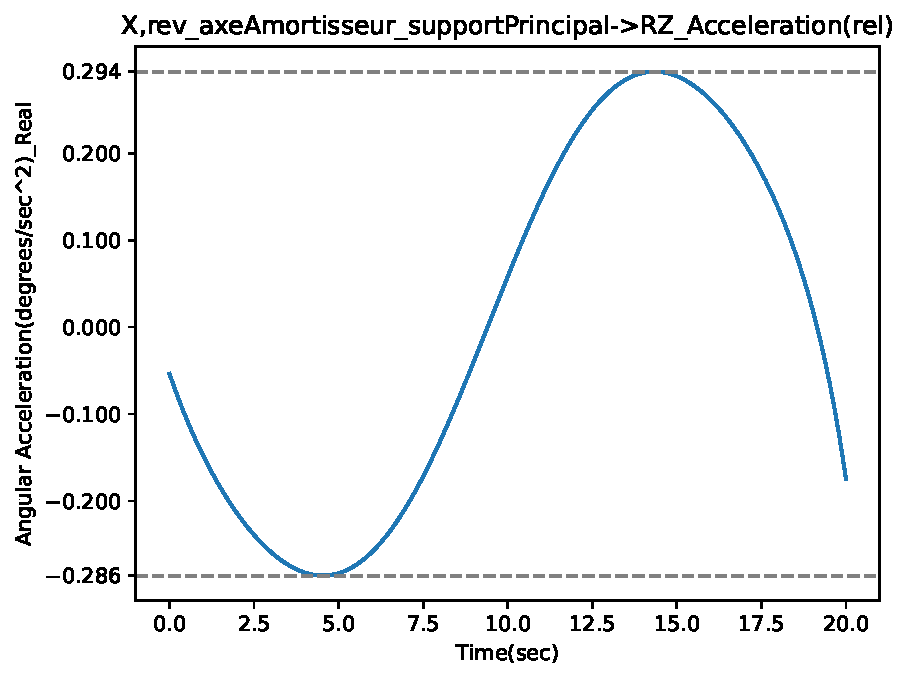
\includegraphics[width=\textwidth]{data/amortisseur_axeAmortisseur.pdf}
        \caption{Accélération angulaire}
        \label{fig:accel_main_axis}
    \end{subfigure}
    \caption{Vitesse et accélération angulaire de l'amortisseur}
    \label{fig:rot_vel_accel_axe_principal}
\end{figure}

Les extrema sont:
\begin{center}
    \begin{tabular}{|c|c|c|}
        \hline
        & Vitesse & Accélération\\
        \hline
        Minimum: & \( \SI{-6,935}{\deg\per\second} \) & \( \SI{-0.286}{\deg\per\second\squared} \)\\
        \hline
        Maximum: & \( \SI{-5.022}{\deg\per\second}\) & \( \SI{0.294}{\deg\per\second\squared} \)\\
        \hline
    \end{tabular}
\end{center}

Comme la fonction décrivant l'accélération est la dérivée de la fonction décrivant la vitesse, on peut observer que les extrema de l'accélération correspondent aux points d'inflexion de la vitesse.

Pour cette même raison, sur les intervales où l'accélération est décroissante, la fonction de la vitesse angulaire est convexe. Quand l'accélération est croissante, la fonction de la vitesse est concave.

On peut observer ces correspondance en superposant les graphes de vélocité et d'accélération angulaire, et en traçant deux verticales, respectivement au minimum et au maximum d'accélération (fig~\ref{fig:combined_vel_accel}).
\begin{figure}[h]
    \centering
    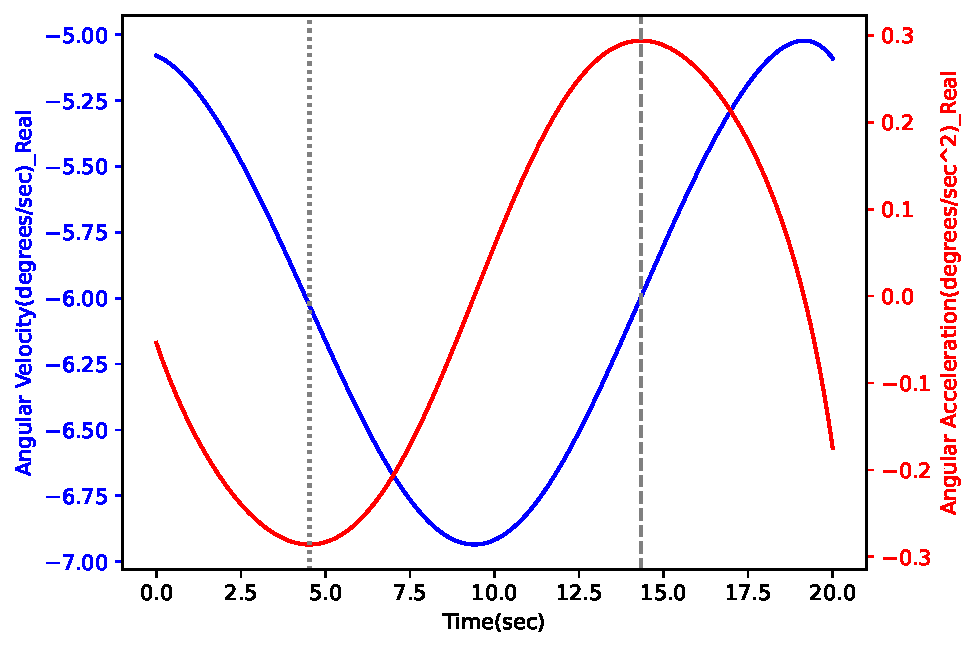
\includegraphics[height=6cm]{data/combined_vel_accel.pdf}
    \caption{Graphe de vitesse et d'accélération angulaire combinés}
    \label{fig:combined_vel_accel}
\end{figure}


\section{Commentaires}
La vitesse angulaire initiale (resp. l'accélération angulaire initiale) n'est pas nulle car, pour cette simulation, nous forçons instantanément la vitesse du vérin à \(\SI{2,7}{\meter\per\second}\). Ce n'est pas réaliste car l'accélération du vérin serait infinie. Il faudrait en réalité appliquer une force, qui se traduirait par une accélération du vérin, qui provoquerait une augmentation progressive de de tout le système au départ d'une vitesse nulle (et vice versa pour les valeurs finales, lorsque le train est presque rentré).

\end{document}